\section{Layer Stackup}
This \acs{PCB} is a two layer PCB. On the top layer the \acs{RF} signals and SMT components are placed. 
The bottom layer is a completed GND layer with some supply traces.
This PCB is produced by my sponsor JLCPCB \footnote{\url{https://jlcpcb.com/}}.
Normally, for bigger RF PCB-Designs a 4 layer PCB is used as follows: 

\begin{figure}[ht!]
	\centering
	\includegraphics[width = 15cm]{example-image}
	\caption{Two Layer PCB Stackup}
	\label{fig:PCB Layer Stackup}
\end{figure}
\newpage

\section{Coplanar Waveguide Grounded (CPWG)}
In RF PCB-Design applications it is very important, that the trace impedance is matched to 50$\Omega$.
Therefore, different techniques like Microstrip, Stripline or Coplanar Waveguide are used.
This PCB-Design uses the Coplanar Waveguide method. However, the calculation of this technique is not that easy (elliptical integrals etc.). That is why an online calculator \footnote{\url{https://chemandy.com/calculators/coplanar-waveguide-with-ground-calculator.htm}}  \cite{CPWGCalculator.2021} is used.
The original equations are in \cite{transmissionLineDesign} on page 79.

\subsection{RX CPWG Calculation}
	\begin{figure}[ht!]
		\centering
		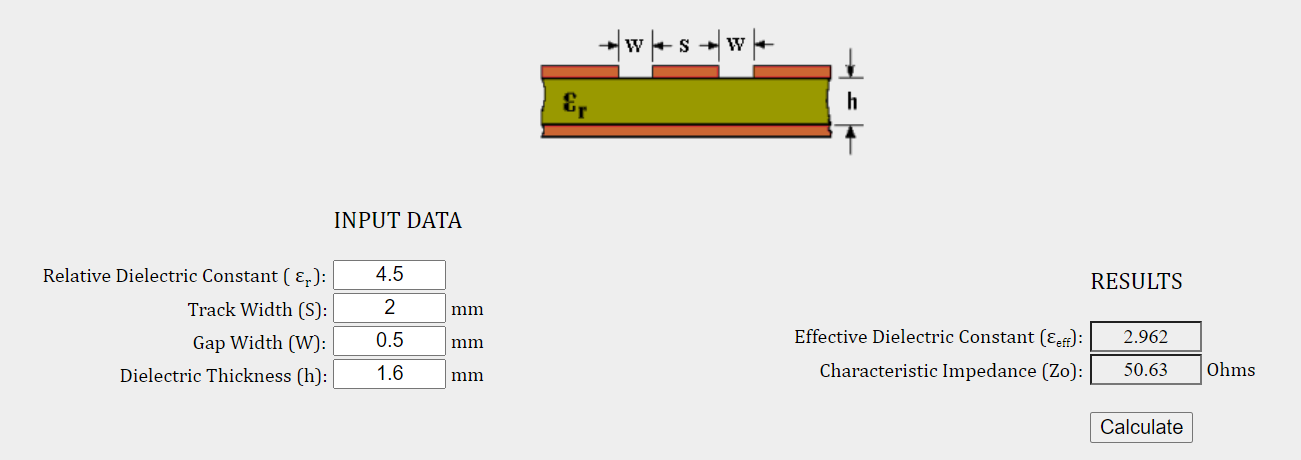
\includegraphics[width = 15cm]{./3_pcb/fig/CPWG_RX}
		\caption{RX CPWG Calculation}
		\label{fig:RX_CPWG}
	\end{figure}

\subsection{TX CPWG Calculation}
	\begin{figure}[ht!]
		\centering
		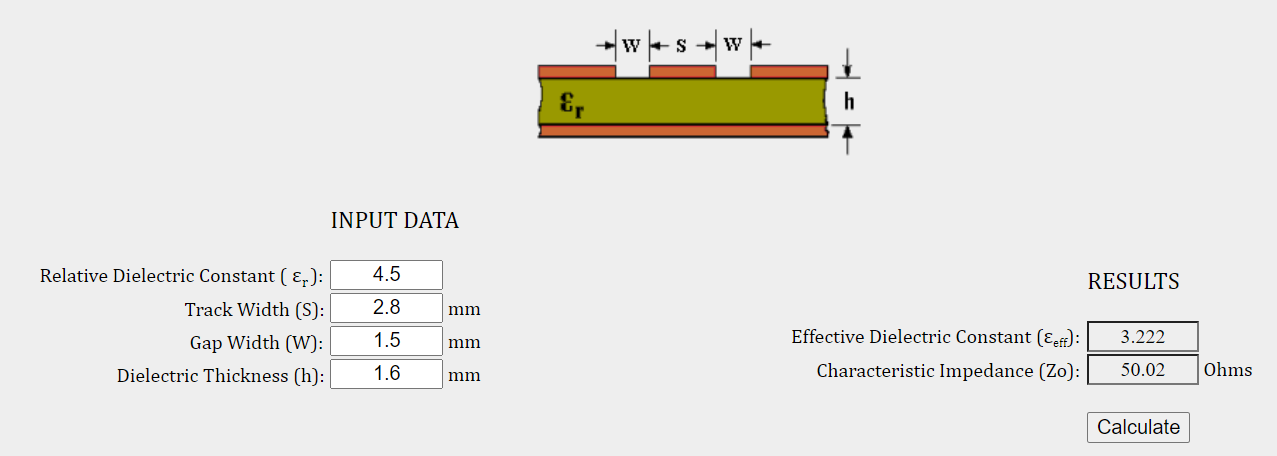
\includegraphics[width = 15cm]{./3_pcb/fig/CPWG_TX}
		\caption{TX CPWG Calculation}
		\label{fig:TX_CPWG}
	\end{figure}

\newpage
\section{Trace corners}	
	ToDo Text
	\begin{figure}[ht!]
		\centering
		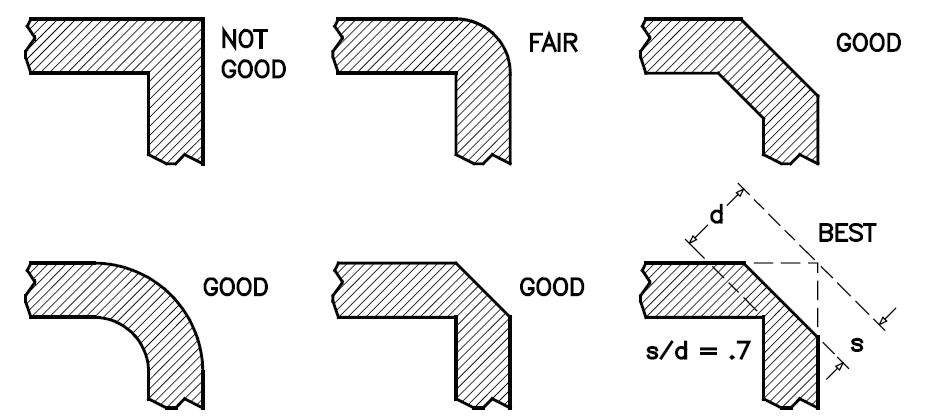
\includegraphics[width = 13cm]{./3_pcb/fig/Trace Corners}
		\caption{Corners in RF traces}
		\label{fig:Corners}
	\end{figure}

\section{3D PCB}	
	\begin{figure}[ht!]
		\centering
		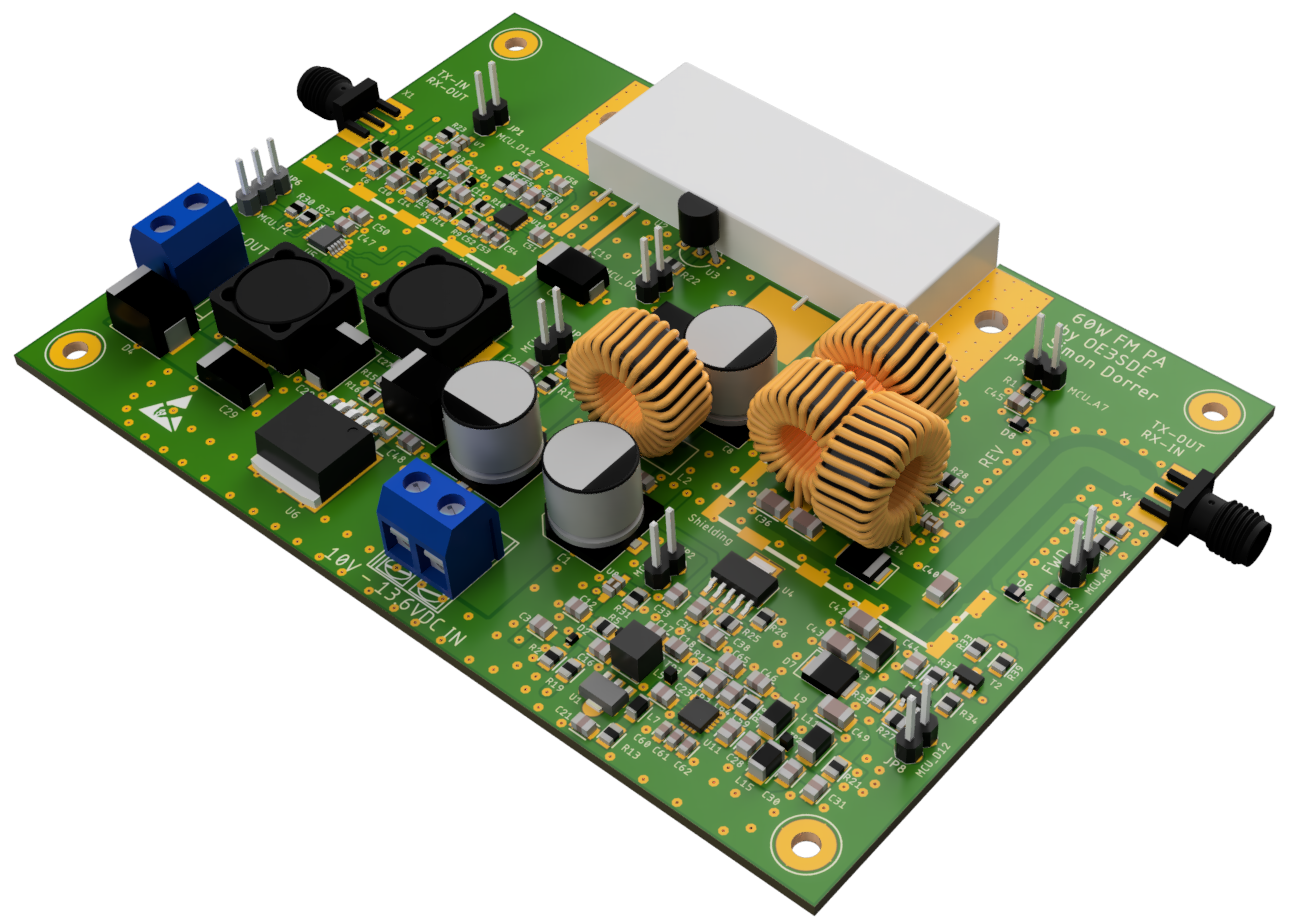
\includegraphics[width = 15cm]{./3_pcb/fig/3D-PCB}
		\caption{Finished \acs{PCB} 3D view}
		\label{fig:3D-PCB}
	\end{figure}

\newpage
\section{2D PCB}	
	\begin{figure}[ht!]
		\centering
		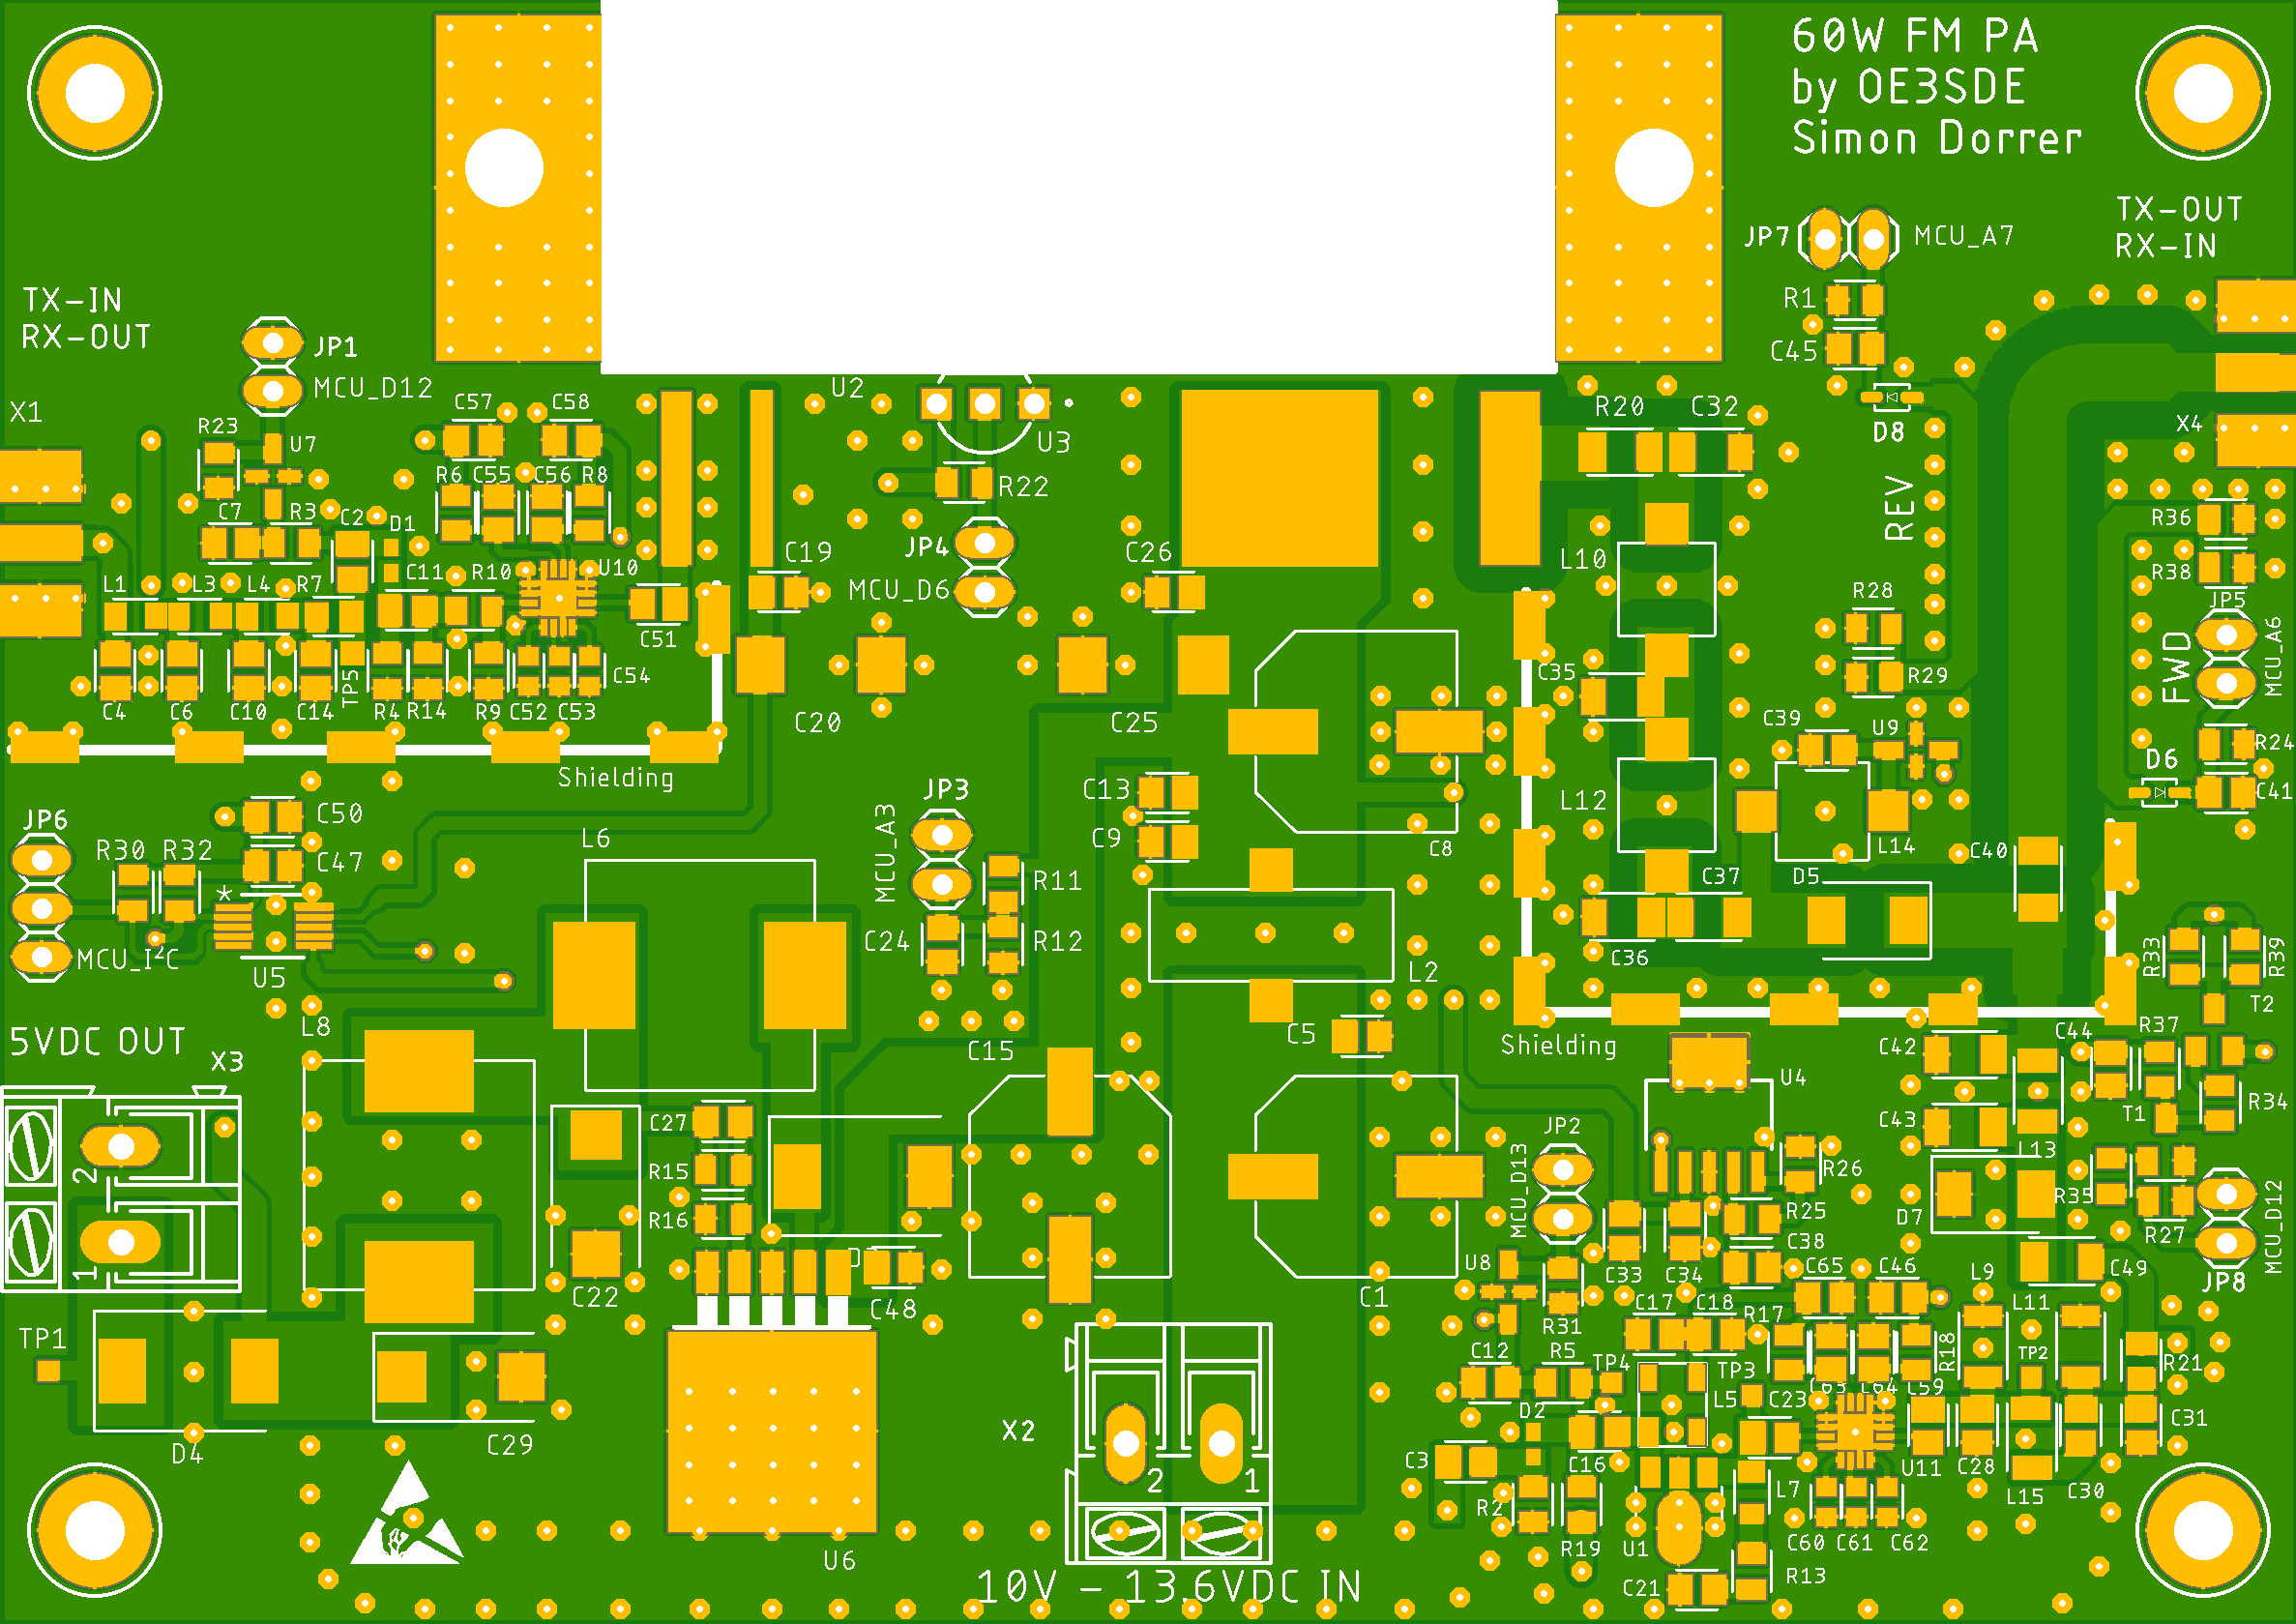
\includegraphics[width = 14cm]{./3_pcb/fig/PCB_Top}
		\caption{Finished \acs{PCB} 2D top view}
		\label{fig:PCB_Top}
	\end{figure}
	\bigskip
	\begin{figure}[ht!]
		\centering
		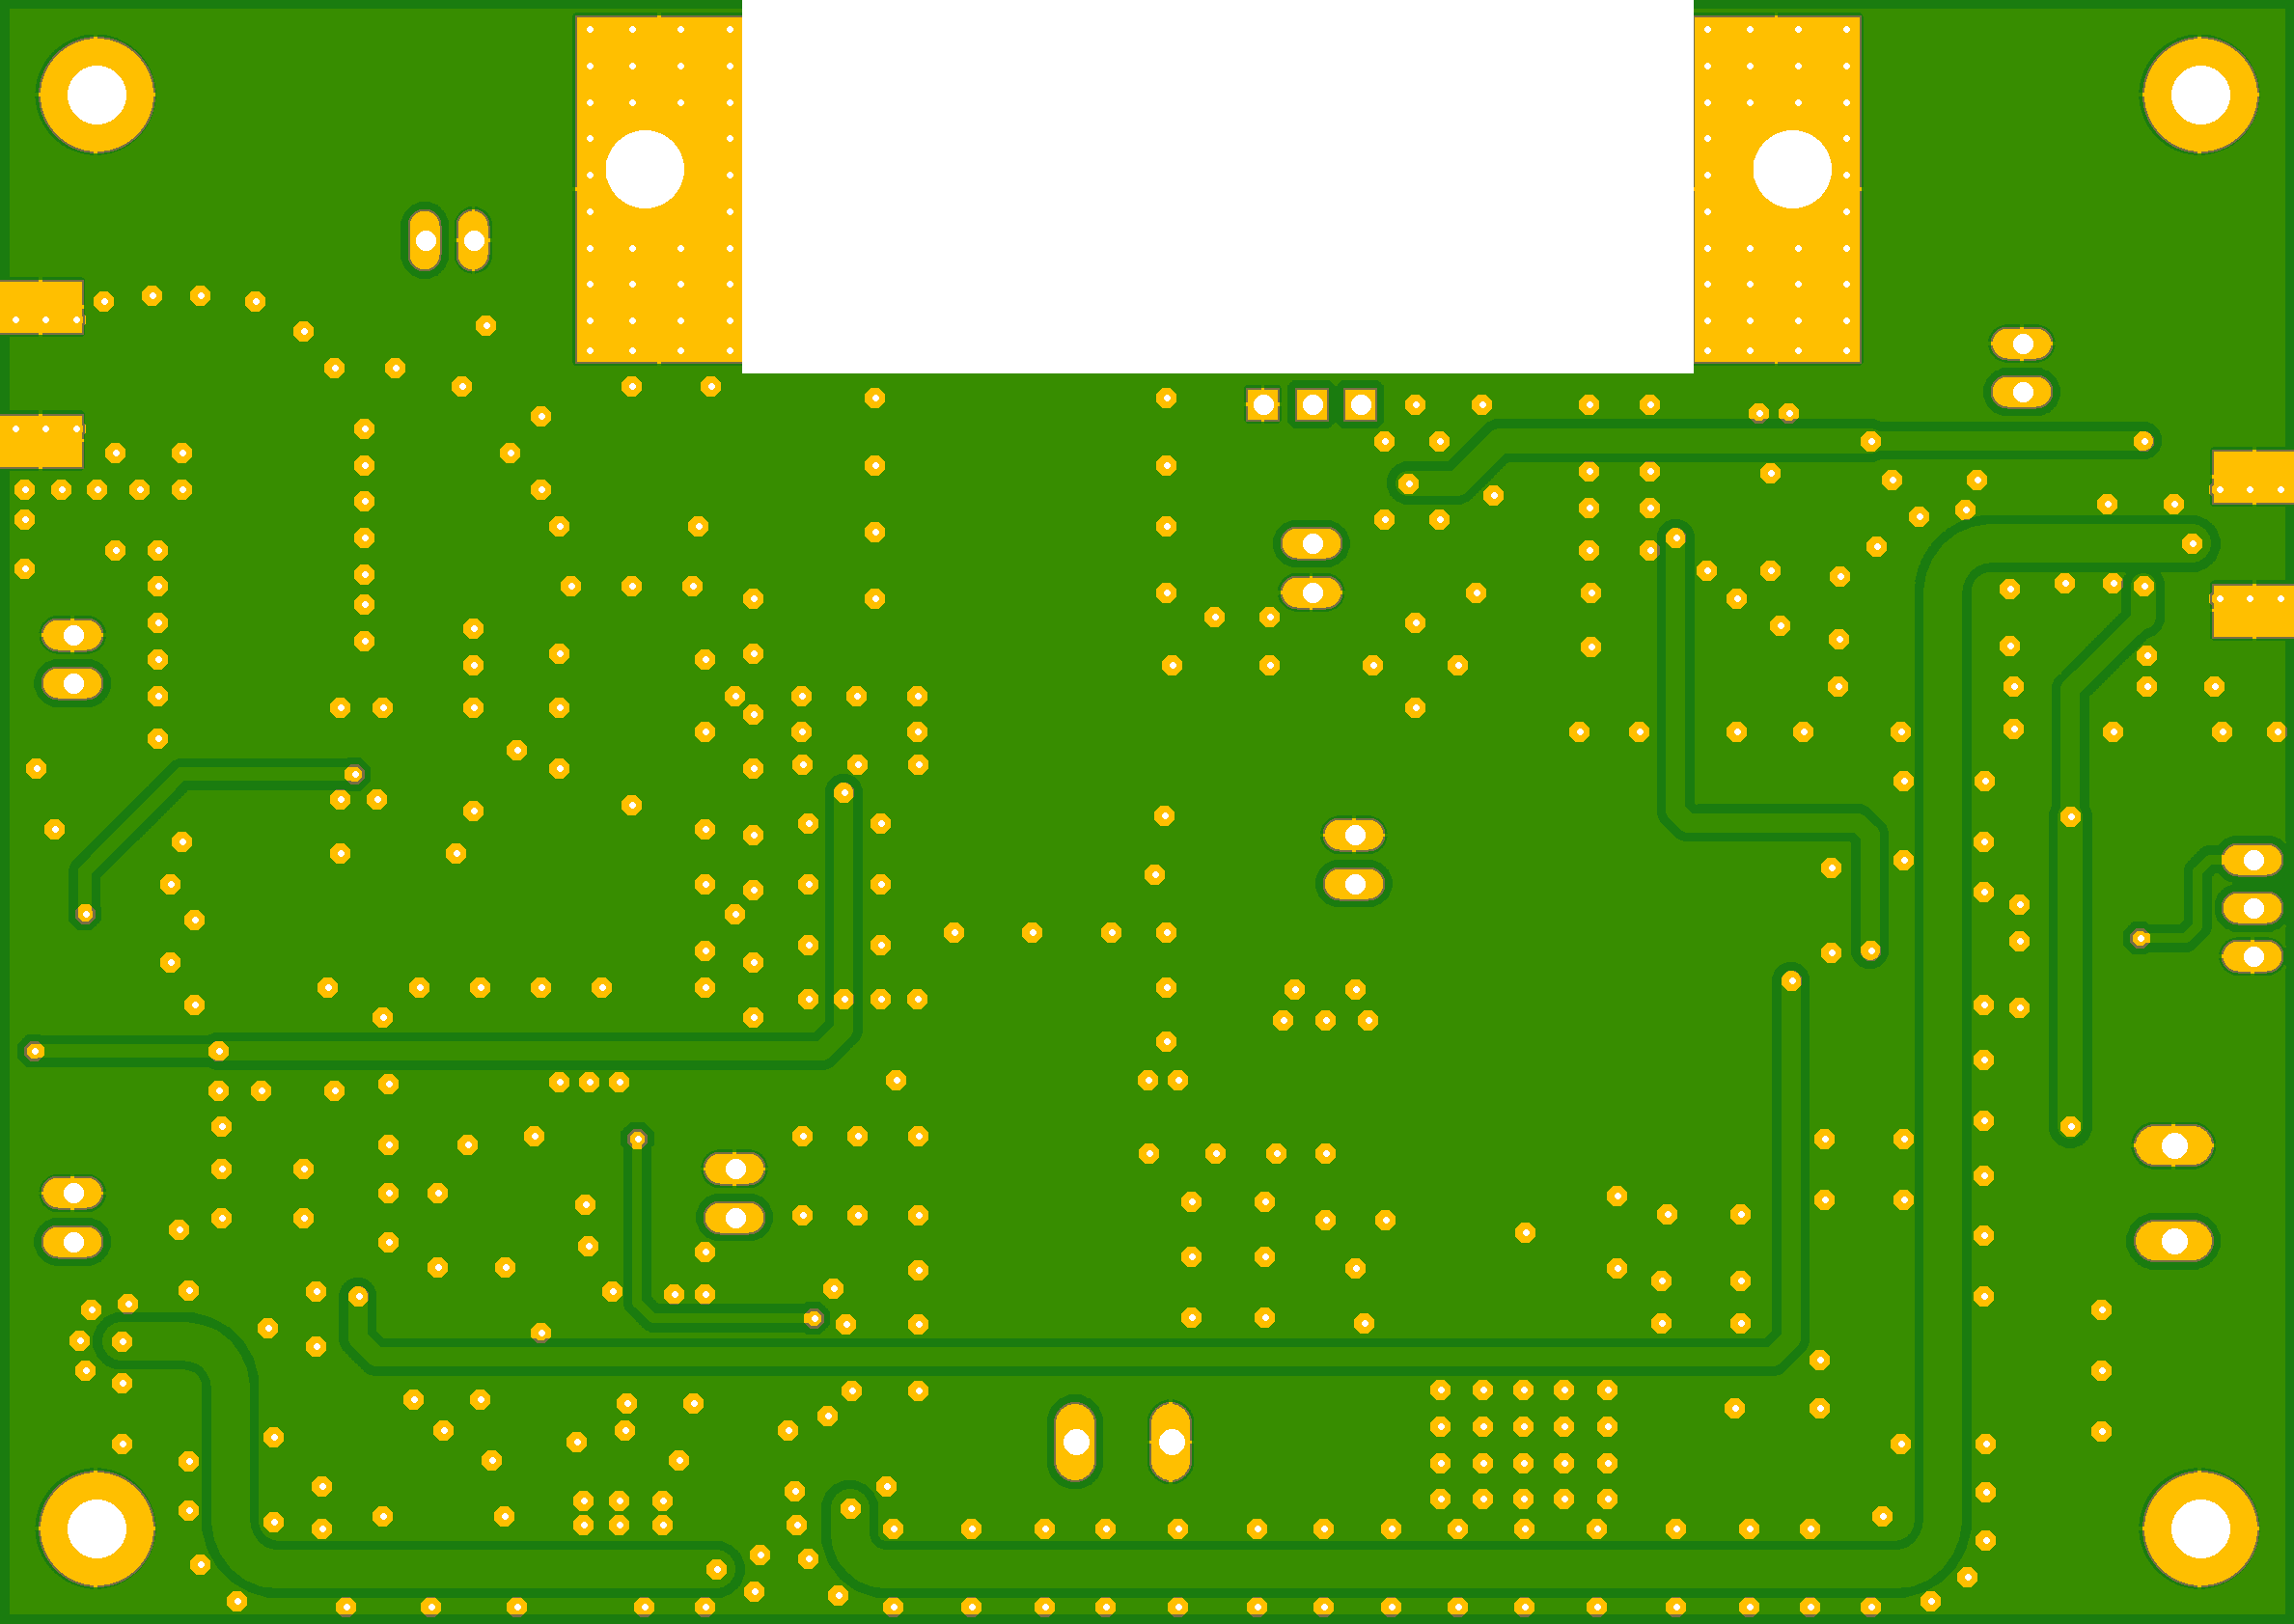
\includegraphics[width = 14cm]{./3_pcb/fig/PCB_Bot}
		\caption{Finished \acs{PCB} 2D bottom view}
		\label{fig:PCB_Bot}
	\end{figure}
\newpage